\documentclass[11pt,a4paper]{article}
\usepackage[margin=24mm]{geometry}
\usepackage{graphicx}
\usepackage{booktabs}
\usepackage{float}
\usepackage{hyperref}
\usepackage{microtype}
\title{Predicting Steel Quality from Production Measurements}
\author{Applied Machine \& Deep Learning (190.015)\\Project P1}
\date{Winter Semester 2026/27}

\begin{document}
\maketitle

\begin{abstract}
This project compares three regression models for predicting a steel-quality
factor from 21 process measurements. The available training file contains
7,642 rows, and the separate test file contains 3,337 rows. Random forest
regression performs best in shuffled five-fold cross-validation
(RMSE $=0.0610\pm0.0019$, $R^2=0.469\pm0.017$) and on the internal
validation split ($R^2=0.428$). All three models have negative $R^2$ on the
provided test file, indicating that the current models do not generalize to
that split. The train--test discrepancy is documented as an open diagnostic,
not attributed to a confirmed cause.
\end{abstract}

\section{Topic and Motivation}
Reliable prediction of product quality from process measurements could help
identify process conditions associated with steel quality and support
data-informed production decisions. This project evaluates whether 21
provided measurements can predict the dataset's continuous quality target,
\texttt{output}.

\section{Related Work}
Machine learning has been applied to steel-property prediction using
production-process and composition data. Millner et al.\ predict several
mechanical properties of steel coils from chemical analyses and production
parameters, illustrating how regression can connect industrial process data
to measured material properties \cite{millner2023}. Their targets and
features are specific to their production dataset; the present course data
does not identify the physical meaning or units of its 21 input columns or
the \texttt{output} target, so the two tasks should not be treated as directly
comparable.

The models selected here provide complementary baselines. Ridge regression
adds an $L_2$ penalty to linear regression and can stabilize estimation when
predictors are correlated \cite{hoerl1970}. Random forests aggregate
decision trees trained with randomized samples and feature choices, allowing
nonlinear relationships without requiring a linear form \cite{breiman2001}.
Support-vector regression uses the support-vector framework to represent
nonlinear functions in a feature space \cite{cortes1995}. Comparing these
families on the same splits helps establish whether a simple linear model,
an ensemble of trees, or a kernel method is most suitable for this dataset.
This project implements that comparison with a leakage-conscious
preprocessing pipeline and reports cross-validation, validation, and
provided-test results.

\section{Methods}
\subsection{Data and preprocessing}
The training CSV has 7,642 rows and 22 numeric columns: 21 inputs
(\texttt{input1}--\texttt{input21}) and the regression target
\texttt{output}. The provided test CSV has 3,337 rows with the same columns.
The recorded data audit found no duplicate rows, missing values, or
non-numeric columns in either original file. Exact duplicate removal and
rows with missing targets are nevertheless handled by the pipeline.

An 80/20 random split of the training file (seed 42) supplies the model
training and internal validation partitions; the provided test file is kept
separate. Numeric outlier fences are calculated as $Q_1-3\,IQR$ and
$Q_3+3\,IQR$ from the training partition and applied by clipping. The
preprocessing pipeline imputes numeric values with the median and
standardizes them; categorical values, if present, are imputed with the
most frequent value and one-hot encoded. Imputation, encoding, and scaling
are fitted as part of each model pipeline using training data only.

The outlier fences are currently calculated once from the full 80\%
training partition before the five-fold cross-validation is run. Therefore,
each cross-validation fold's held-out rows contribute to the fence estimates;
the CV scores may be mildly optimistic with respect to this preprocessing
step. The internal validation and provided test data do not contribute to
those estimates. The input files are already normalized by the course, so
the pipeline does not fit an additional min--max transformation.

\subsection{Models and evaluation}
The comparison uses Ridge regression ($\alpha=1$), a random forest with 200
trees and minimum leaf size 2, and support-vector regression with $C=1$ and
$\epsilon=0.02$. Other model settings use scikit-learn defaults; no
hyperparameter search was performed. Models are compared using five-fold
shuffled cross-validation on the training partition (seed 42). The table
reports the mean and standard deviation across the five fold scores for
RMSE, MAE, and $R^2$. The internal validation and provided-test metrics are
single scores from the fixed 80/20 split and the supplied test file,
respectively; they are not repeated-run averages.

RMSE and MAE measure prediction error, with lower values preferred. $R^2$
measures explained variation relative to predicting the evaluation-set
mean; a negative value means that this baseline would have lower squared
error on that set.

\section{Results}
\subsection{Data inspection}
The original training and test files each contain 22 numeric columns, with
no recorded missing values or duplicate rows. Figure~\ref{fig:hist} shows
the training-file histograms. Figure~\ref{fig:corr} shows the univariate
linear correlations between each input and \texttt{output}; these
correlations describe pairwise association only and do not establish causal
effects or capture general nonlinear relationships.

\begin{figure}[H]
  \centering
  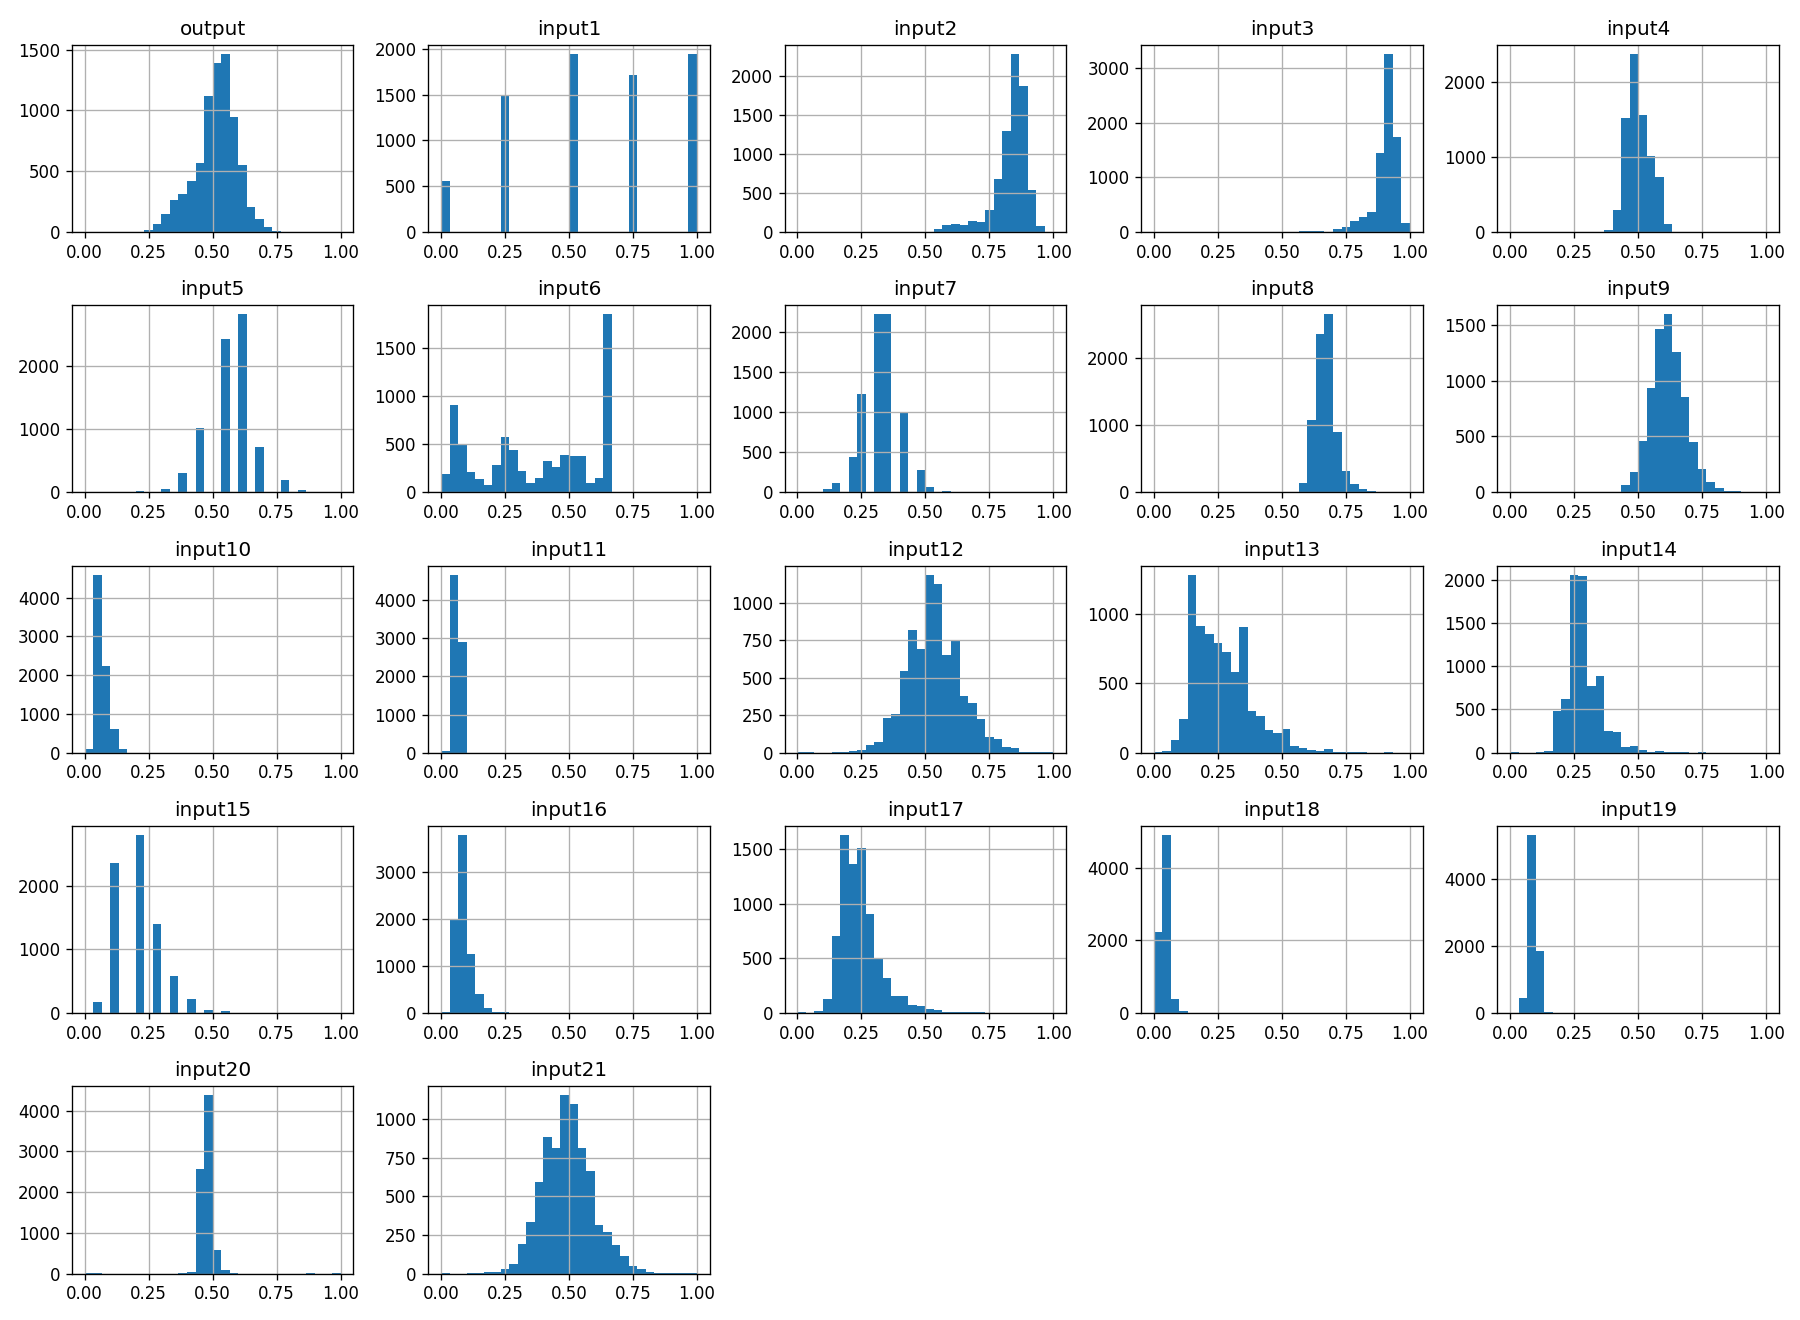
\includegraphics[width=0.82\linewidth]{../results/figures/histograms.png}
  \caption{Histograms of the training data (30 bins).}
  \label{fig:hist}
\end{figure}

\begin{figure}[H]
  \centering
  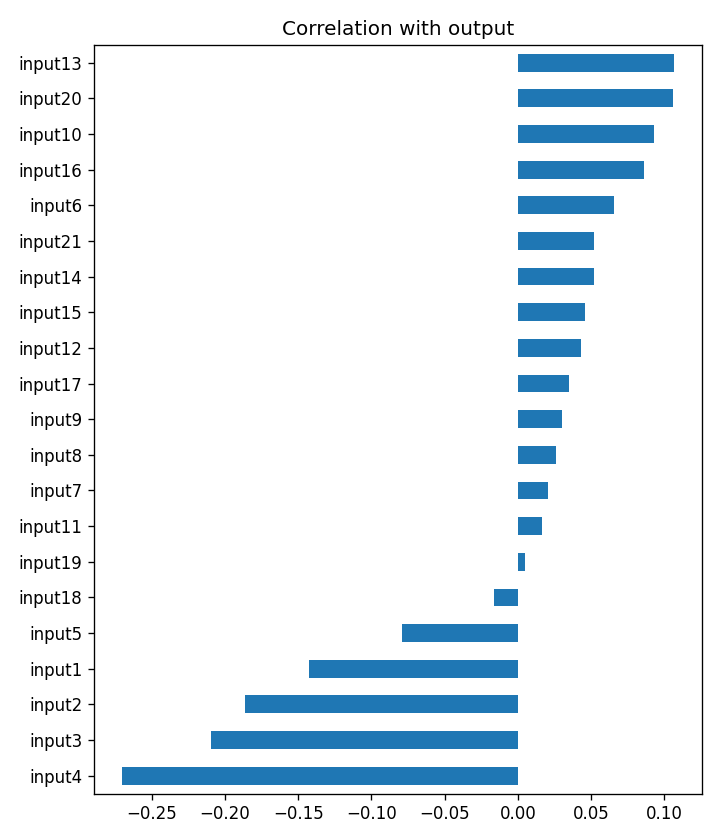
\includegraphics[width=0.68\linewidth]{../results/figures/correlation_with_output.png}
  \caption{Pearson correlations of the numeric inputs with \texttt{output} in the training data.}
  \label{fig:corr}
\end{figure}

\subsection{Cross-validation comparison}
Table~\ref{tab:cv} reports the five-fold cross-validation results. Random
forest has the lowest mean RMSE and MAE and the highest mean $R^2$ among
the three models. Figure~\ref{fig:comparison} visualizes the fold means and
standard deviations; these scores are from five folds of one shuffled split,
not from five independent repetitions of the full experiment.

\begin{table}[H]
  \centering
  \caption{Five-fold cross-validation mean $\pm$ standard deviation on the training partition.}
  \label{tab:cv}
  \begin{tabular}{lccc}
    \toprule
    Model & RMSE & MAE & $R^2$ \\
    \midrule
    Ridge & $0.0751\pm0.0015$ & $0.0581\pm0.0010$ & $0.196\pm0.016$ \\
    Random forest & $\mathbf{0.0610\pm0.0019}$ & $\mathbf{0.0458\pm0.0011}$ & $\mathbf{0.469\pm0.017}$ \\
    SVR & $0.0705\pm0.0020$ & $0.0537\pm0.0021$ & $0.291\pm0.034$ \\
    \bottomrule
  \end{tabular}
\end{table}

\begin{figure}[H]
  \centering
  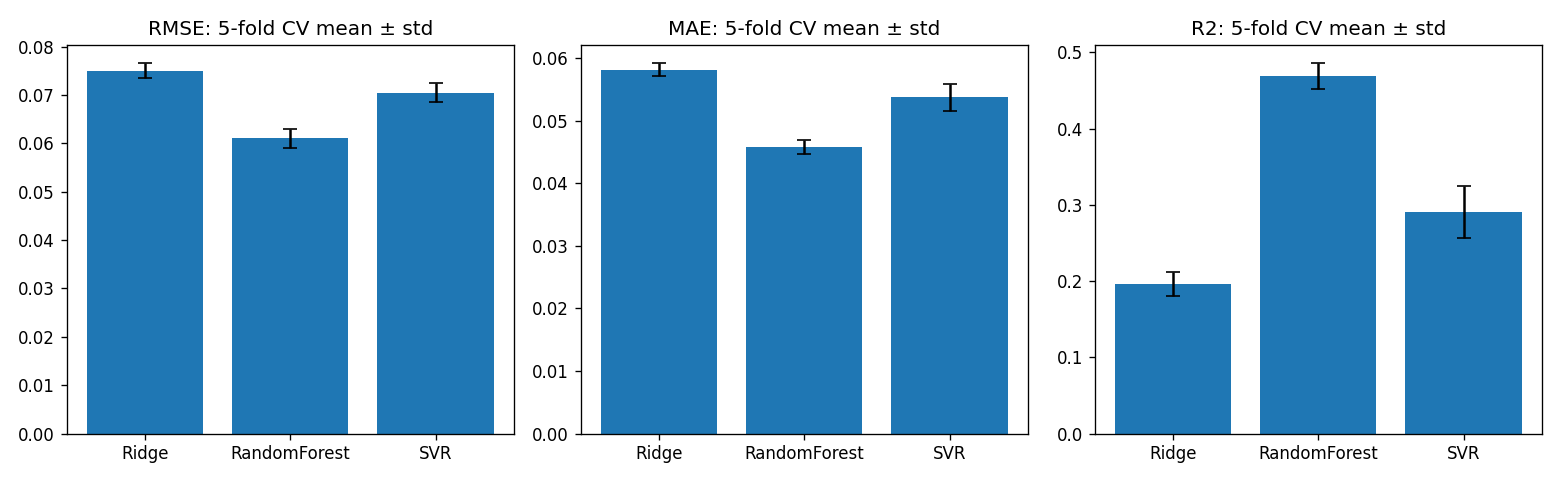
\includegraphics[width=\linewidth]{../results/figures/model_comparison.png}
  \caption{Cross-validation metric means with standard-deviation error bars.}
  \label{fig:comparison}
\end{figure}

\subsection{Validation and provided-test performance}
Table~\ref{tab:holdout} shows single-run results on the internal validation
partition and supplied test file. Random forest is strongest on validation
($R^2=0.428$, RMSE $=0.0617$), consistent with its cross-validation
ranking. Performance changes substantially on the provided test data: all
three $R^2$ scores are negative. SVR has the least negative test $R^2$
($-1.206$) and the lowest test RMSE ($0.1405$), but still performs worse
than predicting the test-set mean under the $R^2$ criterion.

\begin{table}[H]
  \centering
  \caption{Single-split validation and provided-test scores; no standard deviation is available for these single evaluations.}
  \label{tab:holdout}
  \begin{tabular}{lrrrr}
    \toprule
    & \multicolumn{2}{c}{Validation} & \multicolumn{2}{c}{Provided test} \\
    Model & RMSE & $R^2$ & RMSE & $R^2$ \\
    \midrule
    Ridge & 0.0769 & 0.110 & 0.1609 & -1.895 \\
    Random forest & \textbf{0.0617} & \textbf{0.428} & 0.1717 & -2.297 \\
    SVR & 0.0718 & 0.224 & \textbf{0.1405} & \textbf{-1.206} \\
    \bottomrule
  \end{tabular}
\end{table}

The repository's exploratory notes record that both files have column-wise
minimum 0 and maximum 1, while some training and test feature means differ
markedly (for example, \texttt{input3}: 0.90 versus 0.36). This is evidence
of a difference between the supplied files, but it does not establish why
they differ or prove that normalization caused the negative test scores.
The separate scaling/distribution-shift explanation remains a hypothesis
to verify with the dataset provider and a train--test distribution audit.

\section{Limitations}
The physical meaning and units of the anonymized input columns and target
are unknown, which limits interpretation and comparison with published
steel-property studies. Only three untuned models and one fixed
train--validation split were evaluated. The cross-validation outlier fences
are estimated before fold creation, and the negative scores on the supplied
test file show that the current results are not reliable evidence of
generalization to that file.

\section{Conclusion}
Among the evaluated models, random forest performed best in five-fold
cross-validation and on the internal validation split. None of the models
generalized successfully to the provided test file, so no model is ready to
support quality decisions on that data. The next steps are to clarify the
test-file scaling and provenance, estimate preprocessing within each
cross-validation fold, and rerun the comparison before drawing a production
conclusion.

\begin{thebibliography}{9}
\bibitem{millner2023}
G. Millner, M. M\"ucke, L. Romaner, and D. Scheiber,
``Machine learning mechanical properties of steel sheets from an industrial
production route,'' \emph{Materialia}, vol. 30, article 101810, 2023.
\href{https://doi.org/10.1016/j.mtla.2023.101810}{doi:10.1016/j.mtla.2023.101810}.

\bibitem{hoerl1970}
A. E. Hoerl and R. W. Kennard,
``Ridge regression: Biased estimation for nonorthogonal problems,''
\emph{Technometrics}, vol. 12, no. 1, pp. 55--67, 1970.
\href{https://doi.org/10.1080/00401706.1970.10488634}{doi:10.1080/00401706.1970.10488634}.

\bibitem{breiman2001}
L. Breiman, ``Random forests,'' \emph{Machine Learning}, vol. 45,
pp. 5--32, 2001.
\href{https://doi.org/10.1023/A:1010933404324}{doi:10.1023/A:1010933404324}.

\bibitem{cortes1995}
C. Cortes and V. Vapnik, ``Support-vector networks,''
\emph{Machine Learning}, vol. 20, pp. 273--297, 1995.
\href{https://doi.org/10.1007/BF00994018}{doi:10.1007/BF00994018}.
\end{thebibliography}

\end{document}
